\section{Parte I}

\subsection{Problema}

\par Se solicita implementar un algoritmo para una integracion adaptativa, esta consiste en aproximar la integral L(f) dividiendo la integral en subintervalos, esta definida en entre los intervalos [a,b] y se realiza la  división de intervalo de m=(a+b)/2. Para este laboratorio la funcion a evaluar es (1):

\begin{equation}
	L(f) = \int_{a}^{b} 2^{x} - 4x\cdot dx
\end{equation}

\par Se debe determinar la cantidad de iteraciones segun una toleracia de error \textit{tol}, además obtener el error obtenido en la ultima iteración. Los intervalos [a,b] y la tolerancia son ingresados como parametros.

\par Para el desarrollo del calculo de la integral se deben utilizar 3 formas de calculo de integral: 

\begin{enumerate}
	\item Trapecios simples
	\item Integracion de Simpson 1/3
	\item Integracion de Simpson 3/8
\end{enumerate}

\par Para poder realizar los calculos se debe tener un buen conocimiento de como funcionan estos métodos. Al final ya obtenidos los resultados de la integral, iteraciones y error de cada método, se debe incluir gráficas y tablas de evalucacion de errores, comparando los resultados de cada método anteriormente mencionado y que conclusiones se puede sacar al respecto de los resultados.

\newpage

\subsection{Solución}

\par Para poder realizar el algoritmo, se analizó cuales son los datos que necesita el algoritmo como parametros, para ello se solicita al usuario ingresar los intervalos de la integral [a,b] y la tolerancia de error que indica hasta donde se debe ejecutar el programa.

\par Ya ingresados los parametros el programa, el algoritmo debe entregar como resultado las iteraciones y errores de cada uno de los 3 métodos. Para ello se llama a 3 funciones las cuales son los métodos nombrados, estas deben entregar el resultado de cada uno de los métodos. Las funciones descritas se realizaron de la siguiente forma:

\subsubsection{Trapecios Simples}

\par Para trapecios simples se divide la integral en dos, aplicando la regla del trapecio (2):

\begin{equation}
	I = (b-a)\cdot\frac{(f(b) + f(a))}{2}
\end{equation}

\par La regla se aplica 3 divisiones: tomando como parametros a y b,otra tomando a y m (m=(a+b/2)) y la ultima m y b. El error será la resta de cada uno de los valores de estas divisiones por 10. Se realizará esto recursivamente hasta que el error sea menor que le tolerancia indicada.

\subsubsection{Regla de Simpson}

\par Para Simpson se realiza de la misma forma que con trapecio, la única diferencia es la forma en que se divide la integral, existen dos formas:  Simpson 1/3 (3) y Simpson 3/8 (4). Para simpson 3/8 se toma h= (b - a)/3, ya que la función se tabula con cuatro puntos de igual distancia h y formando tres subintervalos.

\begin{equation}
	I = (b-a)\cdot\frac{f(a)+ 4f((a+b)/2) + f(b)}{6}
\end{equation}
\begin{equation}
	I = (b-a)\cdot\frac{f(a)+ 3f(a+h) + f(a+2h) + f(b)}{8}
\end{equation}

\subsection{Resultados}

\par En esta sección entregaremos cada uno de los resultados obtenidos al aplicar cada uno de los métodos en matlab.

\subsubsection{Primera prueba}

\par Para la primera prueba se ingresó de parámetros a y b los valores de 0 y 1 y como tolerancia de error de $10^{-10}$. Con la que se obtuvo los siguientes resultados.

\begin{table}[htp]
	\centering
	\begin{tabular}{ |c|c|c|c|}
		\hline
		\textbf{Método} & \textbf{Aproximación} & \textbf{Error} & \textbf{Iteraciones} \\
		\hline
		Trapecio & -0.557304 & $6.9 \cdot 10^{-11}$ & 4.095  \\
		\hline
		Simpson 1/3 & -0.557304 & $4.4 \cdot 10^{-11}$ & 63  \\
		\hline
		Simpson 3/8 & -0.557304 & $4.4 \cdot 10^{-11}$ & 63 \\
		\hline
	\end{tabular}
	\caption{Tabla de resultados para la primera prueba}
	\label{tab:tab3}
\end{table}

\par A continuación se deja en evidencia el gráfico que se obtuvo al ejecutar el programa en matlab, los cuales nos ayudan a entender el comportamiento de cada uno de los métodos ocupados para esta parte del laboratorio.

\begin{figure}[!ht]
	\centering
	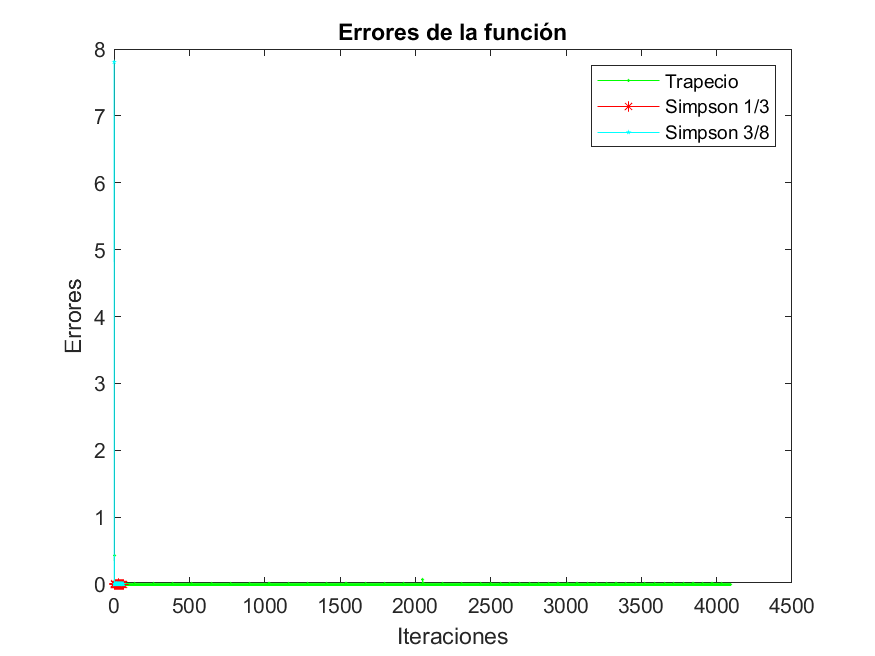
\includegraphics[scale=0.7]{Imagenes/erroresFuncion.png}
	\caption{Resultado de las aproximaciones de la prueba 1}
	\label{fig:ej}
\end{figure}


\subsubsection{Segunda Prueba}

\par Para la segunda prueba se cambio los parámetros iniciales: a=2 y b=7, junto con una tolerancia de $10^{-8}$. Con esto se obtuvo los siguientes resultados.

\begin{table}[htp]
	\centering
	\begin{tabular}{ |c|c|c|c|}
		\hline
		\textbf{Método} & \textbf{Aproximación} & \textbf{Error} & \textbf{Iteraciones} \\
		\hline
		Trapecio & 88.894188 & $8.7 \cdot 10^{-9}$ & 12.787  \\
		\hline
		Simpson 1/3 & 88.894185 & $8.6 \cdot 10^{-9}$ & 251  \\
		\hline
		Simpson 3/8 & 8.894185 & $8.6 \cdot 10^{-9}$ & 251 \\
		\hline
	\end{tabular}
	\caption{Tabla de resultados para la segunda prueba}
	\label{tab:tab3}
\end{table}


\begin{figure}[!ht]
	\centering
	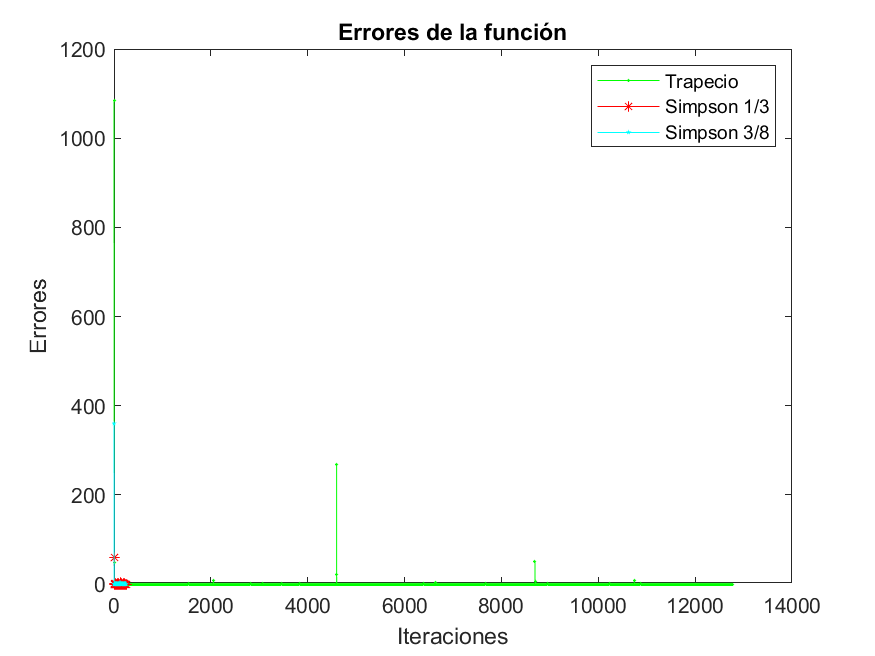
\includegraphics[scale=0.8]{Imagenes/erroresFuncion2.png}
	\caption{Resultado de las aproximaciones de la prueba 2}
	\label{fig:ej}
\end{figure}

\newpage

\subsubsection{Tercera Prueba}

\par Para la tercera prueba se cambio los parametros iniciales: a=1 y b=4, junto con una tolerancia de $10^{-3}$. Con esto se obtuvo los siguientes resultados.

\begin{table}[htp]
	\centering
	\begin{tabular}{ |c|c|c|c|}
		\hline
		\textbf{Método} & \textbf{Aproximación} & \textbf{Error} & \textbf{Iteraciones} \\
		\hline
		Trapecio & -9.799697 & $4.8 \cdot 10^{-4}$ & 105  \\
		\hline
		Simpson 1/3 & -9.802113 & $7.8 \cdot 10^{-5}$ & 11  \\
		\hline
		Simpson 3/8 & -9.802113 & $7.8 \cdot 10^{-5}$ & 11 \\
		\hline
	\end{tabular}
	\caption{Tabla de resultados para la tercera prueba}
	\label{tab:tab3}
\end{table}

\begin{figure}[!ht]
	\centering
	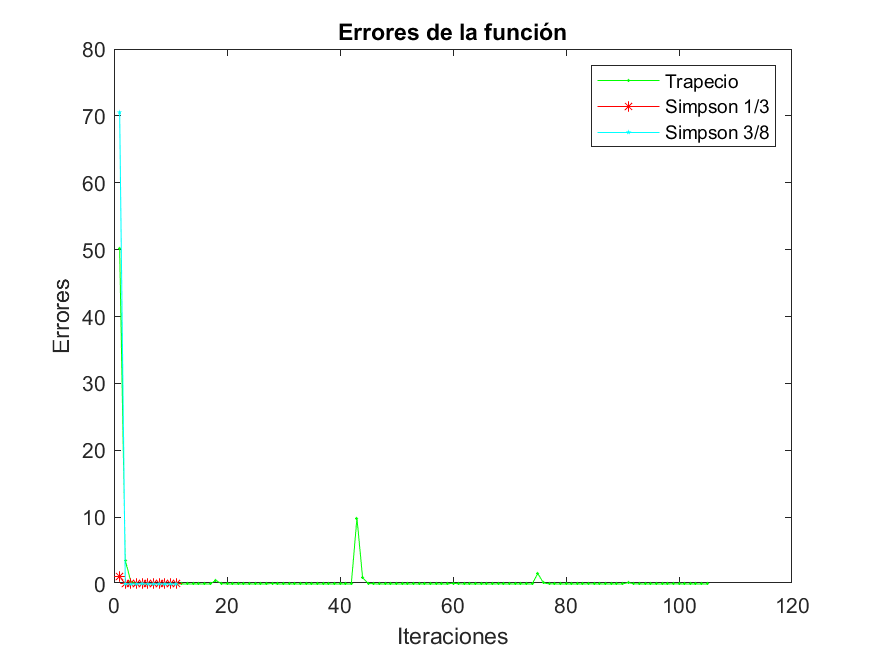
\includegraphics[scale=0.8]{Imagenes/erroresFuncion3.png}
	\caption{Resultado de las aproximaciones de la prueba 3}
	\label{fig:ej}
\end{figure}


